\documentclass[a4paper]{article}
\usepackage[top=1in, bottom=1.25in, left=1.25in, right=1.25in]{geometry}
\usepackage{amsmath}
\usepackage{multicol}
\usepackage{graphicx}
\usepackage[utf8]{inputenc}
\usepackage[english]{babel}
\setlength{\parskip}{0.03cm plus4mm minus3mm}
\RequirePackage{ltxcmds}[2010/12/07]

\usepackage{hyperref}
%opening
\title{MQAM system}

\begin{document}
	
	\maketitle
	
\section{Functional Description}
	
MQAM system is composed of four blocks: a transmitter, a receiver, a communication channel and a block that performs a Bit Error Rate (BER) measurement. The schematic representation of the system is presented in figure \ref{MQAM_system_block_diagram}.

\begin{figure}
	\centering
	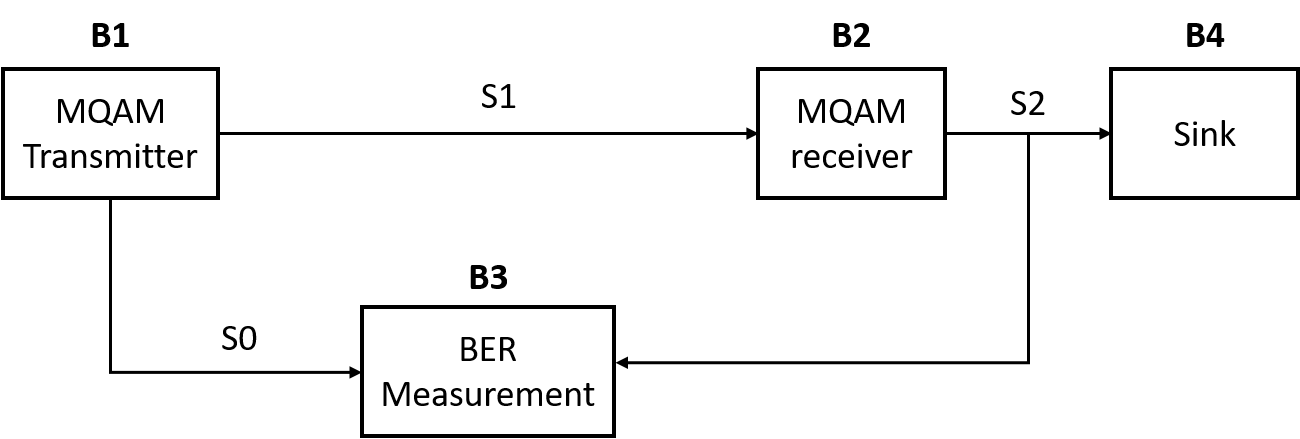
\includegraphics[width=0.8\textwidth]{MQAM_system_block_diagram}
	\caption{Schematic representation of the MQAM system.}\label{MQAM_system_block_diagram}
\end{figure}

%\subsection*{MQAM transmitter}
%
%A complete description of the MQAM transmitter either block by block or as a whole can be found in the \textit{lib} repository. 
%
%This block generates one optical signal. It can also output the binary signal that is used to perform a BER measurement.
%
%\subsection*{Communication channel}
%
%The communication channel has only thermal noise.
%
%\subsection*{MQAM receiver}
%
%The MQAM receiver is a homodyne receiver. 

%\subsection*{BER measurement block}
\end{document}